\documentclass{article}
\usepackage[utf8]{inputenc}
\usepackage[spanish]{babel}
\usepackage{lmodern}
\renewcommand*{\familydefault}{\sfdefault}
\usepackage{graphicx}
\usepackage{titling}
\usepackage{geometry}
\usepackage{setspace}
\usepackage{tikz}
\usepackage{eso-pic}
\usepackage{ragged2e}
\usepackage{hyperref}
\usetikzlibrary{calc}
\usepackage{fancyhdr}
\usepackage{float}
\usepackage{amsmath}

\geometry{
    a4paper,
    total={170mm,257mm},
    left=2.05cm,
    top=3.5cm,
    bottom=30mm,
}

\newcommand{\vcentered}[1]{\begingroup\setbox0=\hbox{#1}
    \parbox{\wd0}{\box0}\endgroup}

% Borde de página
\AddToShipoutPictureBG{
    \begin{tikzpicture}[remember picture,overlay]
        \draw[line width=1pt] ($(current page.north west) + (1cm,-1cm)$) rectangle ($(current page.south east) + (-1cm,1cm)$);
    \end{tikzpicture}}

\begin{document}
    \begin{titlepage}
        \begin{picture}(0,0)
            \put(-20,-70){
\includegraphics[scale=.1]{ipn.png}}
        \end{picture}
        \begin{picture}(0,0)
            \put(320,-50){
\includegraphics[scale=.5]{escom.png}}
        \end{picture}
        \vspace{3cm}
        \begin{spacing}{2}
        \begin{center}
            {\huge \textit{\textbf{Instituto Politécnico Nacional \\ 
                        Escuela Superior de Cómputo \\ 
                        Profesor:  \\  Andres Garcia Floriano \\
                        Alumno: \\ Hernández Jiménez Erick Yael \\ Patiño Flores Samuel \\ Robert Garayzar Arturo \\ 
                        5BV1 \\ 
                        Practica :  \\ Complejidad de datos }}}
        \end{center}
        \end{spacing}       
    \end{titlepage}
    
    %Pie de página
    \pagestyle{fancy}
    \fancyhf{}
    \fancyfoot[C]{\thepage} 
    \renewcommand{\headrulewidth}{0pt} 
    \newpage
    \tableofcontents
    \newpage
    \section{Introducción}
    En el presente trabajo se utilizó un conjunto de datos con el objetivo de mejorar la calidad del mismo mediante dos técnicas clave: la reducción del desbalance de clases y la eliminación de valores perdidos. El desbalance de clases es un problema común en los datasets, especialmente en aquellos que involucran predicción o clasificación, y puede afectar significativamente la precisión de los modelos. \\
   
    
    Para mitigar este problema, se aplicaron estrategias para equilibrar las clases de manera que los resultados del análisis sean más confiables y representativos. Además, se eliminaron los valores perdidos presentes en el dataset para evitar sesgos y asegurar que los algoritmos utilizados operen con datos completos y consistentes.
   
    \section{Desarrollo}
    
    La primera gráfica refleja el desbalance natural del conjunto de datos, donde hay significativamente más personas que ganan menor igual 50K que mayor 50K al año. Este desbalance es común en datos reales y puede causar que los modelos de aprendizaje automático se inclinen a predecir la clase mayoritaria, afectando su capacidad de identificar correctamente la clase minoritaria. Para abordar este problema, se aplican técnicas como SMOTE, que equilibran las clases generando ejemplos sintéticos de la clase minoritaria, lo que mejora el rendimiento predictivo del modelo.
    
    \begin{figure}[H] 
    	\centering
    	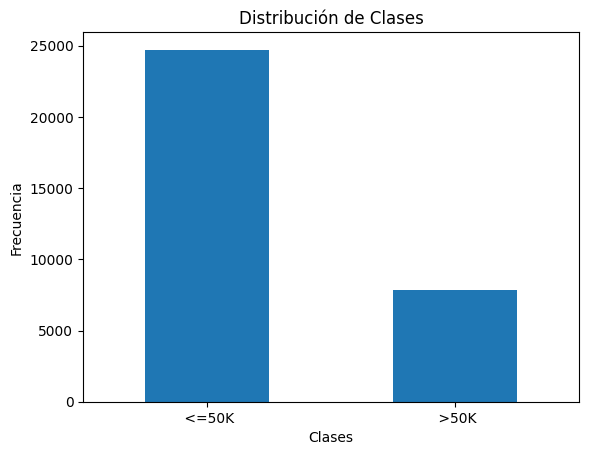
\includegraphics[width=0.5\textwidth]{output_1.png} 
    	\caption{Con cambio significativo.} 
    \end{figure}
    
    Aquí podemos ver como logramos balancear de manera efectiva las clases, y reducir ese gran desbalance que existía previamente, nos ayudamos de la técnica SMOTE para realizar este proceso
    
    \begin{figure}[H] 
    	\centering
    	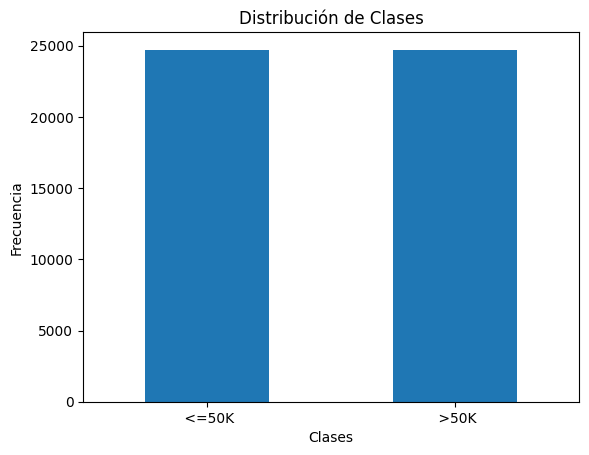
\includegraphics[width=0.5\textwidth]{output_2.png} 
    	\caption{Sin cambio significativo.} 
    \end{figure}
    
    \section{Conclusiones} 
    
    \textbf{\Large Hernández Jiménez Erick Yael:} \\
    
    Una vez realizado el preprocesamiento del set de datos, se pueden destacar la siguiente conclusión: se debe analizar el efecto de cada herramienta que se usará para balancear o manejar los valores nulos ya que un manejo deliberado de estas conllevara errores en la interpretación del set resultante y que puede afectar completamente al análisis posterior o procesamiento por machine learning \\
    
    \textbf{\Large Patiño Flores Samuel:} \\
    
    En esta práctica, se abordaron dos problemas comunes en el análisis de datos: los datos desbalanceados y los datos faltantes. Para tratar el desbalanceo en las clases, se aplicó la técnica SMOTE, que permitió generar ejemplos de la clase minoritaria, evitando el sesgo hacia la clase mayoritaria. En cuanto a los datos faltantes, se utilizó imputación, lo que evitó la pérdida de información valiosa al reemplazar los valores ausentes con estimaciones basadas en los datos disponibles. \\
    
    \textbf{\Large Robert Garayzar Arturo:} \\
    
    La aplicación de técnicas para reducir el desbalance de clases y eliminar los valores perdidos permitió mejorar la calidad del conjunto de datos utilizado. Estas acciones resultaron en un dataset más equilibrado y libre de inconsistencias, lo cual es esencial para obtener resultados más precisos y confiables en modelos de análisis y predicción. Al reducir el sesgo que podría generarse por el desbalance de clases y asegurar que los datos estén completos, se logró una base más sólida para futuros análisis, lo que contribuirá a generar modelos más robustos y generalizables. Este proceso destacó la importancia de la preparación de datos como un paso fundamental en cualquier proyecto de ciencia de datos. \\
    
    
\end{document}
